\documentclass{article}

\usepackage{amsmath}
\usepackage{url}
\usepackage{graphicx}
\usepackage{float}
\usepackage{amsthm}
\usepackage[a4paper, margin=1.5in]{geometry}
\usepackage{amssymb}
\usepackage{enumerate}

\theoremstyle{definition}
\newtheorem{definition}{Definition}[section]
\newtheorem{example}{Example}[section]
\newtheorem*{solution}{Solution}

\theoremstyle{plain}
\newtheorem{theorem}{Theorem}[section]
\newtheorem{lemma}{Lemma}[section]
\newtheorem{corollary}{Corollary}[theorem]

\theoremstyle{remark}
\newtheorem*{remark}{Remark}

\renewcommand{\Re}{\operatorname{Re}}
\renewcommand{\Im}{\operatorname{Im}}
\newcommand{\reals}{\mathbb{R}}

\title{Moments and Characteristic Functions\\Instructor's Notes}
\author{Fu Tianwen \and Yao Chaorui \and Zhao Feng}

\begin{document}
	
\begin{titlepage}
	\maketitle
\end{titlepage}
\tableofcontents
\clearpage
\section{Moments}
\subsection{Definition of Moments}
Generally, in math, the $n$-th moment of a real-valued continuous function about center $c$ is: \cite{wiki:moment}
$$
\mu_n=\int_{-\infty}^\infty (x-c)^nf(x)dx
$$
In particular, for probability density functions $f$ (or cumulative density function $F$), the moments are given by
$$ \mu_n' = E[X^n] = \int_{-\infty}^\infty x^ndF(x) = \int_{-\infty}^\infty x^nf(x)dx $$
Also we have the definition of the central moment \cite{wiki:centralMoment}:
$$
\mu_n = E[(X-E[X])^n] = \int_{-\infty}^\infty (x-\mu)^nf(x)dx
$$
Generally central moments are more useful. Not to be confused with mean $\mu$.
\subsection{Description of Moments}
The first moment is the mean of a random variable, i.e. $$\mu=E[X]$$
The second moment is related to the variance of a random variable:
$$ \text{Var}[X] = E[X^2]-{E[X]}^2$$
In fact the variance is just the second central moment:
$$ \text{Var}[X] = \mu_2 = E[(X-E[X])^2]$$
As for the third central moment, a related concept is skewness. Below shows two random variables with the same mean variance however different in skewness\cite{wiki:skewness}:
\begin{figure}[H]
	\centering
	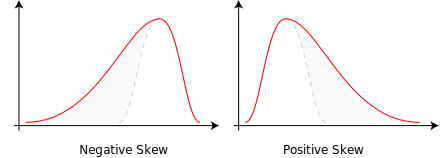
\includegraphics[width=0.8\linewidth]{img/Negative_and_positive_skew_diagrams_(English)}
	\caption{Negative and Positive Skew Diagrams} 
	\label{fig:skewness}
\end{figure}
With all moments up to the order of infinity we can describe the \textbf{characteristics} of a probability distribution.
\section{Characteristic Functions}
\subsection{Moment Generating Functions}
\begin{definition}
	Let X be a random variable with probability density function $f(x)$. If there is a positive number h such that $$ \int_{-\infty}^\infty e^{tx}f(x)dx $$
	exists and is finite for $ −h < t < h$, then the function defined by
	$$M(t) = E[e^{tX}]$$
	is called the moment-generating function of $X$ (or of the distribution of $X$). 
	\textnormal{\cite{psi}}
\end{definition}
The $r$-th moment about the origin can be achieved from the moment generating function by evaluating the $r$-th derivative\cite{pennu}:
$$M^{(r)}(0) = E[X^r] $$
Also notice the relation between the Taylor Expansion and the moments.
\subsection{Characteristic Function}
Notice that $e^{tx}$ is not a "good" function in the sense that it is not bounded and may not converge under some circumstances.
Before going to characteristic functions, we first get acquainted with knowledge of complex numbers:
\subsubsection{Basic information about complex numbers}
Let $z=a+bi$, where $a,b \in \reals$, and $i=\sqrt{-1}$ is the imaginary unit. $z$ is then called a complex number and $a$, $b$ are called the real and imaginary parts of $z$, denoted by $a=\Re(z), b=\Im(z)$ respectively.
(Consider $i$ as rotation by $\frac\pi2$ counterclockwise in the complex plane)\\
The conjugate of a complex number $z=a+bi, a,b\in\reals$ is $\hat{z}=a-bi$, we also define the modulus (or length) of $z$ to be $|z|=z\hat{z}$. Notice that $|z|$ is a non-negative real number.\\
Euler's formula: $$e^{i\theta} = \cos\theta + i\sin\theta$$ The formula comes from Taylor's Series. It also gives rise to the polar representation of a complex number, i.e. $z=re^{i\theta}$, where $r$ is the modulus and $\theta$ is the phase.\\
From this we also have that $|e^{i\theta}| = 1$ for any $\theta$.
\subsubsection{Definition of Characteristic Functions}
\begin{definition}
	Let $X$ be a random variable and denote by $F$ the cumulative distribution function of $X$. The characteristic function $\varphi=\varphi_X$ of $X$ (or of $F$, in which case we also write $\varphi_F$) is defined by \textnormal{\cite{cfms}}
	$$\varphi_X(t):=E[e^{itX}]=\int_{-\infty}^\infty e^{itx}dF(x), t\in\reals$$
\end{definition}
\subsubsection{Basic Properties} 
\begin{theorem}[Uniqueness Theorem \cite{uChicago}]
	Let $X$ be a real random variable with distribution function
	$F$ and characteristic function $\varphi$. Similarly, let $Y$ have distribution
	function $G$ and characteristic function $\psi$. If $\varphi(t) = \psi(t)$ for all $t\in\reals$
	then $F(x) = G(x)$ for all $x \in\reals$.
\end{theorem}
\noindent Properties from here on come from Bisgaard and Zoltan's book \cite{cfms}.
\begin{theorem}
If $X$ and $Y$ are independent random variables then the characteristic function of their sum is $$\varphi_{X+Y}(t) = \varphi_{X}\cdot\varphi_{Y}.$$
\end{theorem}
\begin{corollary}
The product of two characteristic functions is a characteristic function.
\end{corollary}
\begin{remark}
	If $X$ and $Y$ are random variables such that $\varphi_{X+Y} = \varphi_X\cdot\varphi_Y $, then in general we do not conclude $X$ and $Y$ are independent. (See page 13 in \cite{cfms})
\end{remark} 
\begin{theorem}
For any $a,b \in \reals$, $$\varphi_{aX+b}(t)=e^{ibt}\varphi_X(at).$$
\end{theorem}
\begin{theorem}
Every characteristic function $\varphi$ has the following properties:
\begin{enumerate}[(i)]
	\item $\varphi(0)=1,$
	\item $|\varphi(t)|<=1,$
	\item $\varphi(-t)=\overline{\varphi(t)}$
	\item $\varphi$ is continuous on $\reals$
\end{enumerate}
\end{theorem}
\begin{theorem}[Inversion Formula \cite{pte}]
	If $\int_\reals |\varphi(t)| dt < \infty$ then $X$ has bounded continuous density
	$$
	f(x) = \frac1{2\pi} \int e^{-itx}\varphi(t)dt
	$$

\end{theorem}
\subsection{Common Distributions and Their Characteristic Functions}
\begin{table}[ht]
	\caption{Characteristic Functions for Common Distributions\cite{kurser}}
	\centering
	\begin{tabular}{l l l}
		\hline\hline
		Distribution  & PMF/PDF & Characteristic Function\\
		\hline
		Constant $X\equiv a$  & - &  $\varphi_X(t) = e^{iat}.$\\
		Binomial $X\sim Binomial(m,p)$ & $p_X(n) = \binom{n}{m} p^n(1-p)^{m-n}$ &
		$\varphi_X(t) = (pe^{it} + (1-p))^m$\\
		Poisson $X\sim Poisson(\lambda)$ & $p_X(n) = \frac{\lambda ^n}{n!} e^{-\lambda}$ &
		$ \varphi_X(t)=e^{\lambda(e^{it}-1)} $\\
		Exponential $X \sim Exponential(\lambda)$ & $p_X(n) = \lambda e^{-\lambda x}$ &
		$\varphi_X(t)=\frac{\lambda}{\lambda-it}$ \\
		Normal $X\sim N(0,1)$ & $f_X(x) = \frac{1}{\sqrt{2\pi}}e^{-\frac{x^2}{2}}$ &
		$\varphi_X(t)=e^{-\frac{t^2}{2}}$\\
		Normal $Y\sim N(\mu,\sigma ^2)$ & $f_Y(y) = \frac{1}{\sqrt{2\pi}\sigma}e^{-\frac{(y-\mu)^2}{2\sigma ^2}}$ & $\varphi_Y(t)=e^{it\mu-\frac{\sigma^2 t^2}{2}}$
	\end{tabular}
	\label{tbl:charFunc}
\end{table}
%also include some figures here
\section{Examples and Applications of Characteristic Functions}
\begin{example}
	Rain falls on your head at $\lambda$ drops per second on average. What is the distribution of rain drops on your head in two seconds?
\end{example}
\noindent\textbf{Solution.}
Our intuition tells us that it should be $Poisson(2\lambda)$. \\
Let $X,Y$ be two independent $Poisson(\lambda)$ random variables. Let $Z=X+Y$.
Notice that characteristic functions for $X$ (and respectively $Y$) is $\varphi_X(t)=e^{\lambda(e^{it}-1)}$.
Therefore we have $\varphi_Z(t)=\varphi_{X+Y}(t)=(\varphi_X(t))^2=e^{2\lambda(e^{it}-1)}$. 
By uniqueness of characteristic functions we know that $Z\sim Poisson(2\lambda)$.
\begin{remark}
	By similar ideas, one can show that the sum of two independent poisson random variables has a possion distribution with an expectation of the sum of both expectations.
\end{remark}
\begin{example}
	$X_1\sim N(\mu_1,\sigma_1^2), X_2\sim N(\mu_2,\sigma_2^2).$ $X_1,X_2$ are independent. Distribution of $Y=X_1+X_2$?
\end{example}
\noindent\textbf{Solution.}
Similarly to last example $$\varphi_{Y}(t)=\varphi_{X_1+X_2}(t)=e^{it\mu_1-\frac{\sigma_1^2 t^2}{2}}\cdot e^{it\mu_2-\frac{\sigma_2^2 t^2}{2}}$$
Therefore we have $$\varphi_Y(t)=e^{it(\mu_1+\mu_2)-\frac{(\sigma_1^2+\sigma_2^2)t^2}{2}}$$
which implies that $Y\sim N(\mu_1+\mu_2,\sigma_1^2+\sigma_2^2)$
\begin{example}[Central Limit Theorem\cite{waterloo}]
	If $X_i$ are independent identically distributed random variables with $E[X_i] = \mu, Var[X_i] = \sigma^2$ , then $S_n^* = \frac1{\sigma\sqrt n}\sum_{i=1}^n(X_i-\mu)$ converges weakly to $N(0, 1)$.
\end{example}
\noindent\textit{Warning: The proof is not rigorous and serves only for intuitively demonstrating the usage of Characteristic Functions. See the references\cite{waterloo,nus} for detailed proofs.}
\begin{lemma}
	For any random variable $X$ with $E[X]=0,Var[X]=1$, we have $\varphi_X(t)=1-\frac12t^2+o(t^2)$.
	\label{lem:clt}
\end{lemma}
\begin{proof}
	Directly from the definition and Taylor Series we have
	$$\varphi_X(t)=E[e^{itX}]=E[1+itX+\frac{1}{2}i^2t^2X^2+o((tX)^2)]$$
	By linearity of expectation,
	$$\varphi_X(t)=E[1]+itE[X]-\frac{1}{2}t^2E[X^2]+o(t^2)$$
	Also
	$$E[X^2]=Var[X]-(E[X])^2=1$$
	Therefore $$\varphi_X(t)=1-\frac{1}{2}t^2+o(t^2)$$
\end{proof}
\noindent Now with Lemma \ref{lem:clt} we denote the characteristic function of $\frac{X_i-\mu}{\sigma}$ by $\varphi(t)$, then  $\varphi(t)=1-\frac12t^2+o(t^2)$. Therefore the characteristic function of $S_n^*$ is 
$$\varphi^n(t/\sqrt{n})=[1-\frac{t^2}{2n}+o(t^2/n)]^n$$
Take $n\to\infty$ and we get the characteristic function of $\lim\limits_{n\to\infty}S^*_n$
$$\varPhi(t)=\lim\limits_{n\to\infty}\varphi^n(t/\sqrt{n})
=\lim\limits_{n\to\infty}[1-\frac{t^2}{2n}]^n=e^{-\frac{t^2}2}$$
Therefore $\lim\limits_{n\to\infty}S_n^*$ converges to $N(0,1)$.

\begin{lemma}[Parseval identity\cite{kurser}]
F(A) and G(A) are probability measures on a real line;
$\phi(t)=\int_{-\infty}^{\infty}e^{itx}F(dx)$ and $\psi(t) = \int_{-\infty}^{\infty} e^{itx}G(dx)$ are their characteristic functions. Then the Parseval Identity is as follows:
$$\int_{-\infty}^{\infty}e^{-ity}\phi(t)G(dt) = \int_{-\infty}^{\infty}\psi(x-y)F(dx).$$
\end{lemma}
\begin{proof}
    By the definition of characteristic functions, we have:
    $$e^{-ity}\phi(t) = \int_{-\infty}^{\infty} e^{it(x-y)}F(dx)$$
    Integrating it w.r.t. G(A), we get:
    $$\int_{-\infty}^{\infty}e^{-ity}\phi(t) G(dt) = \int_{-\infty}^{\infty}\int_{-\infty}^{\infty} e^{it(x-y)}F(dx)G(dt)$$
    Using Fubini's Theorem, we get:
    $$\int_{-\infty}^{\infty}\int_{-\infty}^{\infty} e^{it(x-y)}F(dx)G(dt) = \int_{-\infty}^{\infty}\int_{-\infty}^{\infty} e^{it(x-y)}G(dt)F(dx) = \int_{-\infty}^{\infty}\psi(x-y)F(dx)$$
\end{proof}
\medskip

\bibliographystyle{ieeetr}
\bibliography{bibliography}
\end{document}
